In this section, the layer is described in terms of the hardware and software design. Specific implementation details, such as hardware components, programming languages, software dependencies, operating systems, etc. should be discussed. Any unnecessary items can be ommitted (for example, a pure software module without any specific hardware should not include a hardware subsection). The organization, titles, and content of the sections below can be modified as necessary for the project.

\subsection{Layer Hardware}
The Music Filter Layer has two major components: The circuit that filters the audio, and the Arduino board that converts the incoming music signal into voltages for the motors.

\subsection{Layer Operating System}
Since the Arduino is a micro-controller, it does not require any operating system to run. All code is put into the firmware of the device.

\subsection{Layer Software Dependencies}
This layer does not need any overlying software to run. It can run independent of software.

\subsection{Subsystem 1: Music Filter}
The Music filter circuit is built with many components that modify the incoming audio signal. It has four main parts: the virtual ground, pre-Amplifier, filters, and power amplifier. The schematic also shows other parts, but they provide no effect to the audio. 

\begin{figure}[h!]
	\centering
 	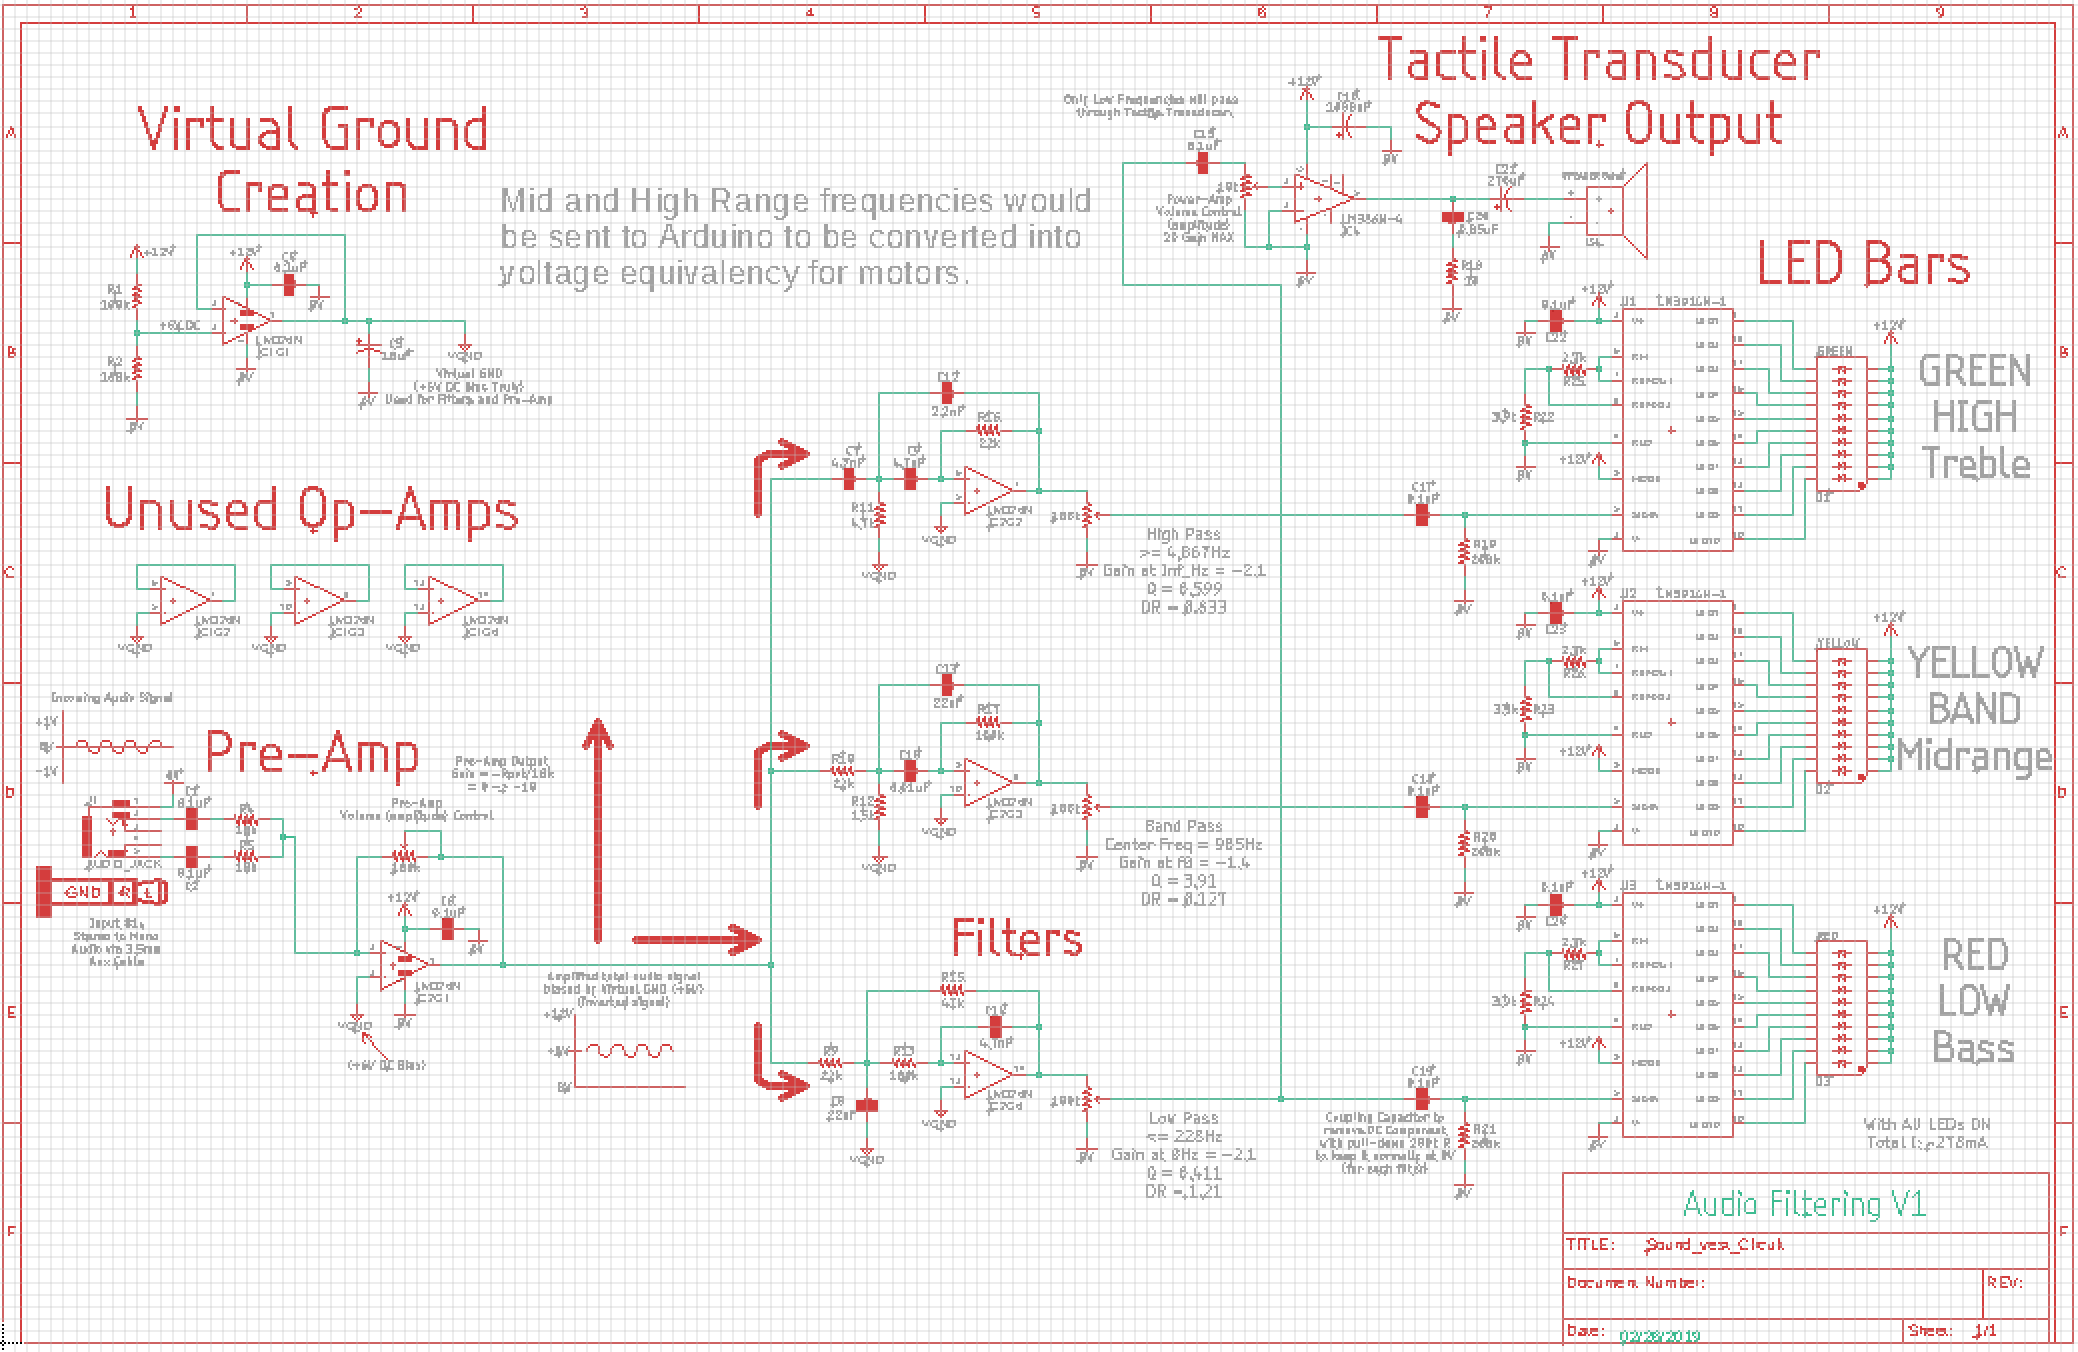
\includegraphics[width=0.8\textwidth]{images/audio_sch}
 \caption{Music Filter Schematic}
\end{figure}

\subsubsection{Subsystem Hardware}
The four main parts to this subsystem are the virtual ground, pre-amplifier, filters, and power-amplifier.

\subsubsection{Subsystem Operating System}
No operating system is needed in this subsystem.

\subsubsection{Subsystem Software Dependencies}
No software dependencies are needed in this subsystem.

\subsubsection{Subsystem Programming Languages}
No programming languages are needed in this subsystem.

\subsubsection{Subsystem Data Structures}
Audio is being sent from the raspberry pi to the filtering circuit through a 3.5mm audio jack. Signal is weak and is first boosted by the pre-amplifier to get the signal to line level. After the signal is filtered into a low, mid, and high range, it passes through a power amplifier that is able to boost the signal even more for the tactile transducer.

\subsubsection{Subsystem Data Processing}
The main portion of the circuit is the filtering of the audio. Audio is separated into a low, mid, and high range of frequencies and then sent to its corresponding outlet. Low frequencies will pass through a power amplifier and then into a speaker capable of producing low frequency rumbles. Mid and high range frequencies are passed on to the Arduino to be converted to voltages for the motors in the next layer. 

\subsection{Subsystem 2: Arduino}
The Arduino Uno micro-controller accepts the filtered signal from the circuit and converts the frequency to voltage in real time.

\begin{figure}[h!]
	\centering
 	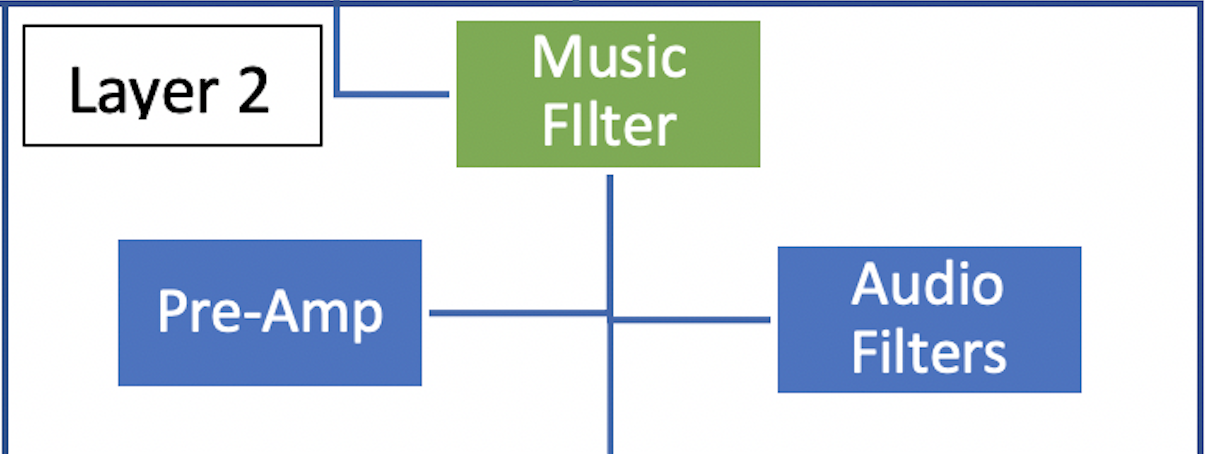
\includegraphics[width=0.8\textwidth]{images/subsystem2}
 \caption{Music Filter Layer Subsystem}
\end{figure}

\subsubsection{Subsystem Hardware}
The only hardware used are the Arduino Uno micro-controller, copper wires, and vibrating mini motors discs.

\subsubsection{Subsystem Operating System}
Since the Arduino is a micro-controller, it does not require any operating system to run. All code is put into the firmware of the device.

\subsubsection{Subsystem Software Dependencies}
The Arduino Uno requires an open-source Arduino Software (IDE) to successfully upload code into the firmware.

\subsubsection{Subsystem Programming Languages}
The arduino can run complied C/C++ code along with libraries.

\subsubsection{Subsystem Data Structures}
Audio is being sent from the raspberry pi to the filtering circuit through a 3.5mm audio jack. Signal is then sent directly to the Arduino Uno.

\subsubsection{Subsystem Data Processing}
The main portion of the circuit is the filtering of the audio. Audio is separated into a low, mid, and high range of frequencies and then sent to its corresponding outlet. Low frequencies will pass through a power amplifier and then into a speaker capable of producing low frequency rumbles. Mid and high range frequencies are passed on to the Arduino to be converted to voltages for the motors in the next layer. 
